%!TEX root = ../template.tex
%%%%%%%%%%%%%%%%%%%%%%%%%%%%%%%%%%%%%%%%%%%%%%%%%%%%%%%%%%%%%%%%%%%%
%% chapter2.tex
%% NOVA thesis document file
%%
%% Chapter with the template manual
%%%%%%%%%%%%%%%%%%%%%%%%%%%%%%%%%%%%%%%%%%%%%%%%%%%%%%%%%%%%%%%%%%%%

\typeout{NT FILE chapter2.tex}%

\chapter{System Design and Implementation}
\label{cha:chap_3}


As discussed in Section~\ref{subsec:communication_gap}, the \gls{iopt}-Tools environment provides robust support for modeling, verifying, and generating code for individual controller sub-models specified with \gls{iopt} Petri nets \cite{iopttools, barros2004, RefiningIOPT}. However, a significant limitation arises in distributed control systems, particularly under the \gls{gals} paradigm, where decomposed sub-models require intercommunication \cite{galsactd, Barrosadd}. Current automatic code generation within \gls{iopt}-Tools focuses primarily on the internal logic of each sub-model, leaving the implementation of communication links to be carried out manually. This process is time-consuming, error-prone and poses substantial challenges for debugging and validation.  

The objective of this dissertation is to address this gap by proposing an automated code generation tool capable of analyzing decomposed \gls{iopt} sub-models obtained through the decomposition of \gls{gals} systems in \gls{iopt}-Tools and automatically producing the necessary communication infrastructure code. In doing so, the tool streamlines the development of distributed control systems and ensures efficient and reliable data exchange pathways.  

This chapter presents the design, implementation, and validation of the proposed tool. It begins with an overview of the system architecture, developed as a web-based Application Programming Interface (\gls{api}) integrated within the \gls{iopt}-Tools ecosystem. The chapter then details the transformation pipeline, from model inputs to generated code outputs, and provides a formal specification of the \gls{api} endpoints and parameters. Subsequently, the generated C++ code is analyzed with respect to three communication protocols: \gls{i2c}, \gls{uart}, and \gls{tcp}/\gls{mqtt}. Finally, the chapter outlines the validation methodology used to assess both the correctness and reliability of the tool’s output.  


% ===================================================================
% Section 3.1
% ===================================================================

\section{System Architecture}
\label{sec:design_decisions}

The tool is implemented as a server-side web Application Programming Interface (\gls{api}), an architectural choice that decouples the code generation logic from the end-user's local environment while providing a platform-independent and highly accessible solution. At the core of the system lies a single PHP script, \texttt{api.php}, hosted on a web server, which is responsible for processing all incoming requests\footnote{The complete open-source implementation of the API is publicly available in a Git repository at: \url{https://github.com/dtavares7/Api}}. The overall architectural workflow, depicted in Figure~\ref{fig:api_Workflow}, illustrates the sequence of interactions from the user's request to the delivery of the generated C++ code.

The process begins with the user, or an automated client, constructing a Hypertext Transfer Protocol (HTTP) GET request containing a set of URL parameters. These parameters specify the desired communication protocol (\gls{i2c}, \gls{uart}, or \gls{tcp}/\gls{mqtt}) and its configuration, including details such as slave addresses, baud rates, or topic names, as defined in Section~\ref{sec:api_spec}. Upon receiving the request, the web server, which can be implemented using common platforms such as Apache or Nginx, acts as the public-facing entry point and forwards the request to the \texttt{api.php} script for processing.

Within the PHP script, the input parameters are first parsed and sanitized, then validated against the \gls{api} specification to ensure completeness and correctness. Based on the selected protocol, the script retrieves the corresponding pre-written C++ code template, which contains placeholders for the protocol-specific configuration values. These templates serve as skeletons for each supported communication protocol, enabling modularity and separation of generation logic from code structure. The script dynamically populates the template with the user-provided parameters and assembles the final C++ source code as a string, ready for integration. In cases of missing or invalid parameters, the script generates an HTTP 400 error response with a descriptive message, ensuring robust error handling.

Finally, the generated C++ code is returned to the user within the body of the HTTP response. This output is formatted as a set of functions and definitions specifically designed for direct integration into the \texttt{net\_io.cpp} file produced by the \gls{iopt}-Tools environment. By centralizing the code generation logic on the server and leveraging templates for each protocol, the \gls{api} provides a reliable, repeatable, and platform-independent method to produce communication modules tailored to the user’s system model.

\begin{figure}[h!]
   \centering
   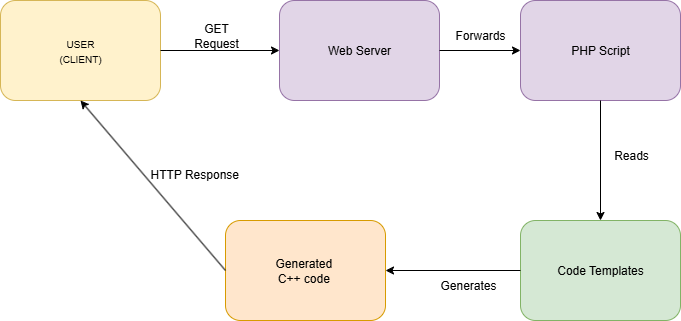
\includegraphics[width=1\textwidth]{Chapters/Figures/apiWorkflow.png}
   \caption{The architectural workflow of the code generation API, illustrating the sequential steps from the user request to the generated C++ code response.}
   \label{fig:api_Workflow}
\end{figure}


% ===================================================================
% Section 3.2   -----------
% ===================================================================

\section{Design Rationale}
\label{sec:design_rationale}


The design and implementation of the code generation tool involved several key decisions regarding its architecture, technology stack, and \gls{api} protocol. Each choice was guided by the objectives of platform independence, usability, and seamless integration with the existing \gls{iopt}-Tools ecosystem, and is discussed below with a rationale comparing alternative approaches.

The tool was conceived as a server-side Web \gls{api} rather than a standalone desktop application or a command-line interface. This architectural decision was motivated primarily by the goals of accessibility and platform independence: a Web \gls{api} can be accessed from any device with a web browser or a standard HTTP client without requiring software installation, whereas desktop applications require separate builds for each operating system, and command-line tools often depend on a specific runtime environment and user familiarity with terminal commands. Furthermore, the Web \gls{api} architecture facilitates seamless integration with the web-based \gls{iopt}-Tools environment, allowing the code generation functionality to be incorporated into the existing front-end workflow. Centralized deployment also simplifies maintenance, as updates and bug fixes applied on the server are instantly available to all users, in contrast to desktop or CLI solutions that require distributing updates to individual installations.

The selection of PHP as the implementation language was a deliberate choice after evaluating alternatives such as Python with Flask or FastAPI, and Node.js with Express. PHP is particularly well-suited for code generation tasks which fundamentally involve sophisticated string manipulation and template processing. Its extensive built-in string handling functions greatly simplify the implementation of the code templating engine, while its server-side simplicity and "shared-nothing" request-response model align naturally with the stateless operation of the \gls{api}. Additionally, PHP is one of the most widely deployed back-end languages, supported by virtually all web hosting providers, which ensures ease of deployment and long-term maintainability. Another important consideration is the future integration of this \gls{api} with the \gls{iopt}-Tools platform, which itself is implemented in PHP; adopting the same language ensures architectural compatibility and a smooth path for integration, allowing the code generation tool to become a native component of the \gls{iopt}-Tools web environment.

Although modern RESTful \gls{api} design often favors \texttt{POST} requests with JSON payloads to handle structured data, a simpler \texttt{GET-based} interface was intentionally chosen for this application. This approach offers practical advantages in usability, debugging, and reproducibility: \texttt{GET} requests can be easily constructed and tested directly in a web browser's address bar, facilitating rapid experimentation and demonstration, and the tool's dedicated help page (\texttt{help.php}) provides additional guidance for users. Since each code generation request is independent, the stateless and idempotent nature of \texttt{GET} requests ensures predictable behavior without the need to maintain the server-side session state. Finally, encapsulating the complete \gls{api} call, including all configuration parameters, within a single URL enhances shareability and allows users to bookmark or distribute specific code generation configurations, as detailed in Section~\ref{sec:api_spec}.

Overall, the combined choice of a server-side Web \gls{api} implemented in PHP with a \texttt{GET}-based interface achieves the project's goals of accessibility, maintainability, and seamless integration. By evaluating alternative approaches and emphasizing usability, the tool provides a robust and user-friendly solution for automated code generation within the \gls{iopt}-Tools ecosystem.



% -------------------------------------------------------------------
% Subsection 3.3 :  ----------- Mapping Model Constructs to Implementation Primitives
% -------------------------------------------------------------------

\section{Mapping Model Constructs to Implementation Primitives}
\label{sec:mapping_constructs}

A critical function of the generation tool is to create a conceptual bridge between the abstract formalism of the decomposed \gls{iopt} Petri net model and concrete primitives of the generated C++ code. This section describes how the \gls{api} systematically translated the high-level constructs of the \gls{gals} extended \gls{iopt} models into tangible programming constructs.

An important mapping concerns event-triggered transitions, which correspond to protocol-specific message transmissions. In the decomposed model, a transition that sends an event to another sub-model is implemented as a conditional block within the sender's \texttt{PutOutputSignals()} or \texttt{OutputSignals()} function. The activation of this transition, represented in code as \texttt{if (events->eventName == 1)}, is directly associated with a function call that transmits a message using the chosen protocol primitive. Examples include \texttt{Wire.write()} for \gls{i2c}, \texttt{MySerial.println()} for \gls{uart}, and \texttt{client.publish()} for \gls{mqtt}.

Another essential mapping involves the Asynchronous Channel (\gls{ac}), which in the abstract model facilitates communication across different clock domains in a \gls{gals} system. In software, this construct is realized through a two-part mechanism. First, an asynchronous reception primitive is used and its form depends on the chosen protocol: an Interrupt Service Routine (\texttt{onReceive}) for \gls{i2c}, polling of the serial buffer (\texttt{MySerial.available()}) for \gls{uart}, or a client callback function for \gls{mqtt}. Second, upon receiving the correct message, this mechanism sets a \texttt{volatile} boolean flag. The flag functions as a safe, memory-mapped bridge between the asynchronous communication domain (where the message arrives) and the synchronous Petri net execution domain, where it is polled within the \texttt{GetInputSignals()} function.

Finally, the transfer of tokens between sub-models is directly mapped to the exchange of message payloads. Concretely, the data or state represented by a token is encoded in the \texttt{slaveMessage}, \texttt{uartMessage}, or \texttt{tcpMessage} parameter of the \gls{api}. The successful reception of this specific payload by the destination controller effectively completes the token transfer and enables the progression of the corresponding Petri net.

Through these mappings, the tool establishes a systematic and consistent correspondence between abstract model constructs and concrete implementation primitives, thereby ensuring that the semantics of \gls{gals} extended \gls{iopt} models are faithfully preserved in the generated code.


% ===================================================================
% Section 3.4: 
% ===================================================================

\section{Application Programming Interface (API) Specification}
\label{sec:api_spec}

This section provides a formal specification of the Application Programming Interface (\gls{api}) for the code generation tool. The \gls{api} is designed to be accessed via HTTP GET requests, with all configuration options passed as URL parameters.
To complement this formal specification and provide a practical, on-demand reference, a dynamic help page was implemented at the \texttt{help.php} endpoint. This page serves as a live user manual that presents a summary of the base endpoint, the required global parameters, and a detailed breakdown of each protocol. For each protocol, it lists all available parameters, indicates whether they are required or optional, specifies their default values, and provides a complete, ready-to-use example URL. This feature is designed to facilitate the ease of use and rapid testing of the \gls{api} directly from a web browser.

The base endpoint for the \gls{api} corresponds to the server location of the main script, as illustrated below:
\begin{verbatim}
    http://<server_address>/api.php
\end{verbatim}

Every \gls{api} request must include three global parameters that define the context for the code generation. These are detailed in Table \ref{tab:global_params}.

\begin{table}[h!]
    \centering
    \caption{Global API Parameters}
    \label{tab:global_params}
    \begin{tabular}{|l|c|p{9cm}|}
        \hline
        \textbf{Parameter} & \textbf{Status} & \textbf{Description} \\ \hline
        \texttt{protocol} & Mandatory & Specifies the communication protocol. Must be one of: \texttt{i2c}, \texttt{uart}, or \texttt{tcp}. \\ \hline
        \texttt{projectName} & Mandatory & A C-identifier compliant string defining the project name, used for function naming in the generated code. \\ \hline
        \texttt{eventName} & Mandatory & A C-identifier compliant string defining the specific event to be handled. \\ \hline
    \end{tabular}
\end{table}

% -------------------------------------------------------------------
% Subsection for each protocol
% -------------------------------------------------------------------
\subsection{Protocol-Specific Parameters}
\label{subsec:protocol_params}

In addition to the global parameters, each protocol requires or accepts a unique set of parameters to configure its behavior according to the protocol needs.

\paragraph{\gls{i2c} Protocol.} For \gls{i2c} communication, the parameters specified in Table \ref{tab:i2c_params} are required.

\begin{table}[h!]
    \centering
    \caption{API Parameters for the \gls{i2c} Protocol}
    \label{tab:i2c_params}
    \begin{tabular}{|l|c|l|p{6cm}|}
        \hline
        \textbf{Parameter} & \textbf{Status} & \textbf{Type} & \textbf{Description} \\ \hline
        \texttt{slaveAddress} & Mandatory & Integer & The 7-bit address of the slave device. Valid range: 8–119. \\ \hline
        \texttt{slaveMessage} & Mandatory & Char / Int & The command byte, which may be specified either as a single ASCII character or as an integer value (0–127). \\ \hline
    \end{tabular}
\end{table}

\paragraph{UART Protocol.} The \gls{uart} protocol interface offers several optional parameters for fine-tuning the serial communication, as detailed in Table \ref{tab:uart_params}.

\begin{table}[h!]
    \centering
    \caption{API Parameters for the UART Protocol}
    \label{tab:uart_params}
    \begin{tabular}{|l|c|l|p{6cm}|}
        \hline
        \textbf{Parameter} & \textbf{Status} & \textbf{Type} & \textbf{Description / Default Value} \\ \hline
        \texttt{serialPort} & Optional & Integer & The hardware serial port to use on the ESP32 (0, 1, or 2). \textbf{Default: 2}. \\ \hline
        \texttt{rxPin\_receiver} & Optional & Integer & The \gls{rx} pin for the device receiving the message. \textbf{Default: 16}. \\ \hline
        \texttt{txPin\_receiver} & Optional & Integer & The \gls{tx} pin for the device receiving the message. \textbf{Default: 17}. \\ \hline
        \texttt{rxPin\_sender} & Optional & Integer & The \gls{rx} pin for the device sending the message. \textbf{Default: 17}. \\ \hline
        \texttt{txPin\_sender} & Optional & Integer & The \gls{tx} pin for the device sending the message. \textbf{Default: 16}. \\ \hline
        \texttt{baudRate} & Optional & Integer & The data transmission rate in bits per second. \textbf{Default: 115200}. \\ \hline
        \texttt{uartMessage} & Optional & String & The message string that triggers the event. \textbf{Default: "trigger\_<eventName>"}. \\ \hline
    \end{tabular}
\end{table}

\paragraph{TCP/MQTT Protocol.} For network communication via \gls{tcp}/\gls{mqtt}, the \gls{api} requires a topic to be specified. Other parameters related to network and broker configuration are optional, with predefined default values that facilitate rapid prototyping and testing. These are listed in Table \ref{tab:tcp_params}.

\begin{table}[h!]
    \centering
    \caption{API Parameters for the TCP/MQTT Protocol}
    \label{tab:tcp_params}
    \begin{tabular}{|l|c|l|p{6cm}|}
        \hline
        \textbf{Parameter} & \textbf{Status} & \textbf{Type} & \textbf{Description / Default Value} \\ \hline
        \texttt{topic} & Mandatory & String & The \gls{mqtt} topic for publishing and subscribing. \\ \hline
        \texttt{clientID} & Optional & String & The unique client identifier for the \gls{mqtt} connection. \textbf{Default: "ESP32\_IOPT"}. \\ \hline
        \texttt{broker} & Optional & String & The address of the \gls{mqtt} broker. \textbf{Default: "broker.hivemq.com"}. \\ \hline
        \texttt{port} & Optional & Integer & The network port for the \gls{mqtt} broker. \textbf{Default: 1883}. \\ \hline
        \texttt{ssid} & Optional & String & The Service Set Identifier (SSID) of the Wi-Fi network. \textbf{Default: "yourNetworkName"}. \\ \hline
        \texttt{password} & Optional & String & The password for the Wi-Fi network. \textbf{Default: "yourNetworkPassword"}. \\ \hline
        \texttt{tcpMessage} & Optional & String & The message payload that triggers the event. \textbf{Default: "trigger\_<eventName>"}. \\ \hline
    \end{tabular}
\end{table}



% ===================================================================
% Section 3.5: 
% ===================================================================

\section{Analysis of Generated Code}
\label{sec:analysis_of_code}

This section presents and analyzes the concrete C++ source code produced by the \gls{api}. The generated code is specifically designed for integration into the \texttt{net\_io.c} file, a standard output of the \gls{iopt}-Tools C code generator that serves as the hardware interface layer. As the \gls{api} generates C++ to leverage modern libraries (e.g., for \gls{i2c} and \gls{mqtt}), it is a mandatory step to rename this file to \texttt{net\_io.cpp} to ensure the C++ compiler is used.

A critical challenge in integrating external communication is bridging the gap between asynchronous events (e.g., the arrival of a network packet or a bus message) and the synchronous, deterministic execution cycle of the Petri net model. To address this, a consistent software design pattern the "asynchronous-to-synchronous bridge"is employed across all generated modules. This pattern uses a \texttt{volatile} boolean flag to safely signal the occurrence of an external event to the main synchronous loop. The following subsections analyze the specific implementation of this pattern for each supported protocol.

\subsection{\gls{i2c}-Based Communication Channel}
The \gls{i2c} protocol is well-suited for communication on a shared bus, following a master-slave paradigm. The \gls{api} generates distinct code for master and slave controllers.

\noindent\textbf{Sample API Call (Slave):}
\begin{verbatim}
?protocol=i2c&projectName=DemoProject&eventName=buttonPress&
slaveAddress=9&slaveMessage=P
\end{verbatim}

The slave controller's code,provided in full in Appendix~\ref{appendix:i2c}, relies on an Interrupt Service Routine (\gls{isr}) for event detection. This is an efficient, event-driven approach where the microcontroller's hardware immediately executes the \texttt{receive\gls{i2c}Event} function upon data arrival, without requiring the main loop to continuously check for messages.

\begin{verbatim}
/*
* PART 1: Place this at the top of your file with the other global 
variables and includes.
*/
#include <Wire.h>
#define I2C_SLAVE_ADDRESS_for_buttonPress 9 // Address for this device
#define CMD_TRIGGER_buttonPress 'P' // Command to activate the event
volatile bool buttonPress_trigger_flag = 0;
void receiveI2CEvent(int byteCount); // Function prototype


/*
* PART 2: Place this inside your 'DemoProject_InitializeIO()' function.
*/
// Start the \gls{i2c} bus as a slave with the defined address
Wire.begin(I2C_SLAVE_ADDRESS_for_buttonPress);
// Register the callback function that will be called when receiving data
Wire.onReceive(receiveI2CEvent);


/*
* PART 3: Place this inside your 'DemoProject_GetInputSignals()' function.
*/
if (buttonPress_trigger_flag == 1) {
events->buttonPress = 1;
buttonPress_trigger_flag = 0; // Reset the flag to fire only once
} else {
events->buttonPress = 0; // Ensure the event is inactive by default
}


/*
* PART 4: Place this at the bottom of your file with the other helper functions.
*/
void receiveI2CEvent(int byteCount) {
if (Wire.available() > 0) {
char command = Wire.read();
if (command == CMD_TRIGGER_buttonPress) {
buttonPress_trigger_flag = 1;
}
}
while (Wire.available() > 0) {
Wire.read();
}
}
\end{verbatim}

The core of the asynchronous-to-synchronous bridge is the volatile bool buttonPress\_trigger\_flag. The \texttt{volatile} keyword is critical: it instructs the compiler not to apply optimizations to this variable, ensuring that every read of the flag in the main loop fetches its true, up-to-date value from memory, which may have been modified at any time by the \gls{isr}. This prevents potential race conditions and ensures the event is reliably detected by the synchronous Petri net logic.

\subsection{UART-Based Communication Channel}
\gls{uart} communication is ideal for point-to-point serial data exchange. Unlike the \gls{isr}-driven \gls{i2c} slave, the \gls{uart} implementation uses polling.

\noindent\textbf{Sample API Call:}
\begin{verbatim}
?protocol=uart&projectName=SystemA&eventName=toggleLED&baudRate=9600
\end{verbatim}

In the code, provided in full in Appendix~\ref{appendix:uart}, the main loop actively checks for incoming data in each cycle by calling \texttt{MySerial.available()}. This polling approach is simpler to implement than ISRs and avoids some complexities of interrupt programming. However, it relies on the Petri net's execution cycle being fast enough to check the serial buffer before it overflows. This presents a classic trade-off in embedded systems: ISRs offer lower latency and higher responsiveness at the cost of complexity, while polling is simpler but can potentially miss events in systems with a slow or variable loop rate.

\begin{verbatim}

/*
* PART 1: Place this at the top of your file with the other global
 variables and includes.
*/
#include <HardwareSerial.h>

// -- \gls{uart} Configuration --
HardwareSerial MySerial(2);
#define RXD2 16
#define TXD2 17

// -- Message and Flag Definitions --
const String message_uart_toggleLED = "trigger_toggleLED";
volatile bool toggleLED_trigger_flag = 0; // flag only for receiving signals

// -- Function Prototypes --
void setupUart_toggleLED();
String receiveDataUart();
void waitMessageUart();

/*
* PART 2: Place this inside your 'SystemA_InitializeIO()' function.
*/
setupUart_toggleLED();

/*
* PART 3: Place this inside your 'SystemA_GetInputSignals()' function.
*/
waitMessageUart();
if (toggleLED_trigger_flag == 1) {
events->toggleLED = 1;
toggleLED_trigger_flag = 0; // Reset the flag to fire only once
} else {
events->toggleLED = 0; // Ensure the event is inactive by default
}

/*
* PART 4: Place this at the bottom of your file with the other helper functions.
*/
void setupUart_toggleLED() {
MySerial.begin(9600, SERIAL_8N1, RXD2, TXD2);
Serial.println("\gls{uart} communication initialized (Receiver).");
}

String receiveDataUart() {
if (MySerial.available()) {
String data = MySerial.readStringUntil('\n');
data.trim();
return data;
}
return "";
}

void waitMessageUart() {
String receivedMessage = receiveDataUart();
if (receivedMessage.length() > 0 && receivedMessage == message_uart_toggleLED) {
toggleLED_trigger_flag = 1;
Serial.println("Correct message received. Flag for 'toggleLED' activated.");
}
}

\end{verbatim}

Despite the different detection mechanism (polling vs. \gls{isr}), the code employs the exact same \texttt{volatile} flag pattern to safely bridge the asynchronous nature of serial data arrival with the synchronous \texttt{GetInputSignals()} function call.

\subsection{TCP/MQTT-Based Communication Channel}
For networked systems, the tool generates code using the \gls{mqtt} protocol, which enables a robust publish-subscribe model. This approach is inherently asynchronous and event-driven.

\noindent\textbf{Sample API Call:}
\begin{verbatim}
?protocol=tcp&projectName=SensorNetwork&eventName=alert&topic=sensors/events
\end{verbatim}

The implementation, provided in full in Appendix~\ref{appendix:tcp}, leverages the \texttt{PubSubClient} library, which uses a callback function (\texttt{callback}) that is automatically executed when a message arrives on a subscribed topic. This is conceptually similar to an \gls{isr} but operates at a higher software level. The same asynchronous-to-synchronous bridge pattern is used to signal the event to the main loop.

\begin{verbatim}
// PART 1: Global scope definitions
#include <WiFi.h>
#include <PubSubClient.h>
volatile bool alert_trigger_flag = 0; // The bridge pattern again

/...

/*
* PART 3: Place inside SensorNetwork_GetInputSignals()
*/
if (alert_trigger_flag) {
events->alert = 1;
alert_trigger_flag = 0;
} else {
events->alert = 0;
}

/*
* PART 4: Place inside SensorNetwork_LoopDelay()
*/
loopDelayTcp(topic_sub_alert);


/*
* PART 5: Helper functions (place at the bottom)
*/
void tcpMqttInitializeIO() {
Serial.begin(115200);
WiFi.begin(ssid, password);
Serial.print("Connecting to WiFi...");
while (WiFi.status() != WL_CONNECTED) {
delay(500);
Serial.print(".");
}
Serial.println("\nWiFi connected!");
client.setServer(mqtt_broker, mqtt_port);
client.setCallback(callback);
}

void reconnect(const char* topic) {
while (!client.connected()) {
Serial.print("Connecting to \gls{mqtt} broker...");
if (client.connect(client_id)) {
Serial.println("connected!");
client.subscribe(topic);
} else {
Serial.print("failed, rc=");
Serial.println(client.state());
delay(5000);
}
}
}

void loopDelayTcp(const char* topic) {
if (!client.connected()) {
reconnect(topic);
}
client.loop();
}

void callback(char* topic, byte* payload, unsigned int length) {
String msg = "";
for (int i=0; i<length; i++) msg += (char)payload[i];
msg.trim();
if (msg == String(message_tcp_alert)) {
alert_trigger_flag = 1;
Serial.println("Correct \gls{tcp} message received. Flag activated for 'alert'.");
}

// In main loop, client.loop() must be called to check for messages
// This call triggers the callback if a message is pending.
\end{verbatim}

A key feature of the generated \gls{mqtt} code is its focus on resilience. Distributed systems must be able to handle network disruptions. The generated code includes a \texttt{reconnect()} function that automatically attempts to re-establish the connection to the Wi-Fi network and the \gls{mqtt} broker if it is lost. This ensures that the controller can recover from transient network failures, making the overall system more robust.

% ===================================================================
% Section 3.6: 
% ===================================================================

\section{Tool Validation}
\label{sec:tool_validation}

  Following the implementation of the code generation tool, a two-stage validation process was conducted to verify its reliability and functional correctness of its output. The first stage focused on testing the \gls{api}'s behavior and robustness against a range of inputs, while the second stage involved empirically validating the generated C++ code on target hardware.

\subsection{API Functionality Testing}
\label{subsec:api_testing}

  The \gls{api} endpoint was systematically tested to ensure its robustness and adherence to the specification described in Section \ref{sec:api_spec}. The methodology involved subjecting the \gls{api} to a series of HTTP GET requests with both valid (positive testing) and invalid (negative testing) parameter sets to verify correct behavior and error handling. A representative sample of these test cases is detailed in Table~\ref{tab:api_test_cases}.

\begin{table}[h!]
\centering
\caption{Representative API Test Cases and Results}
\label{tab:api_test_cases}
\begin{tabular}{|l|p{2.5cm}|p{6cm}|p{3.5cm}|}
\hline
\textbf{Test Type} & \textbf{Description} & \textbf{Sample Input (URL Fragment)} & \textbf{Expected Outcome} \\ \hline
\textbf{Positive} & Valid \gls{i2c} request with all mandatory parameters. & \texttt{?protocol=\gls{i2c}\&projectName=Demo \&eventName=e1\&slaveAddress=8 \&slaveMessage=A} & HTTP 200 OK with syntactically correct C++ code. \\ \hline
\textbf{Positive} & Valid \gls{uart} request using default and custom parameters. & \texttt{?protocol=uart\&projectName=Demo \&eventName=e2\&baudRate=9600} & HTTP 200 OK with syntactically correct C++ code. \\ \hline
\textbf{Positive} & Valid \gls{tcp}/\gls{mqtt} request with a specific topic. & \texttt{?protocol=tcp\&projectName=Demo \&eventName=e3\&topic=dev/test} & HTTP 200 OK with syntactically correct C++ code. \\ \hline
\textbf{Negative} & Missing a mandatory parameter (\texttt{topic} for \gls{tcp}). & \texttt{?protocol=tcp\&projectName=Demo \&eventName=e3} & HTTP 400 Bad Request with a descriptive error message. \\ \hline
\textbf{Negative} & Parameter value outside the valid range (\texttt{slaveAddress} > 119). & \texttt{?protocol=\gls{i2c}\&projectName=Demo \&eventName=e1\&slaveAddress=150} & HTTP 400 Bad Request with a descriptive error message. \\ \hline
\textbf{Negative} & Unsupported protocol name. & \texttt{?protocol=can\&projectName=Demo \&eventName=e4} & HTTP 400 Bad Request with a descriptive error message. \\ \hline
\end{tabular}
\end{table}

  The tests confirmed that the tool consistently produced syntactically correct C++ code for all valid parameter combinations.   In all negative test cases, the \gls{api} correctly identified the input as invalid and returned the expected HTTP 400 status code, confirming the robustness of the input validation and error handling logic.

\subsection{Generated Code Validation}
\label{subsec:code_validation}

  The second stage of validation focused on confirming that the code generated by the tool was not only syntactically correct but also functionally operational in a real-world scenario.

\subsubsection{Testbed Environment}
  A physical testbed consisting of two ESP32-WROOM-32 microcontroller development boards was established. The development environment was the Arduino IDE, utilizing standard libraries such as \texttt{Wire.h} for \gls{i2c}, \texttt{HardwareSerial.h} for \gls{uart}, and \texttt{PubSubClient.h} for \gls{mqtt}. For network tests, the boards connected via Wi-Fi to a local network, which had access to a public \gls{mqtt} broker (HiveMQ). Communication was monitored via the Arduino IDE's serial monitor.

\subsubsection{Validation Procedure and Results}
For each of the three protocols, a pair of sender (Master/Publisher) and receiver (Slave/Subscriber) applications was generated using the \gls{api}.   The code was integrated into a minimal Arduino project, compiled, and uploaded to the two ESP32 boards.   The boards were connected according to the protocol requirements.   The sending device was then triggered to simulate a Petri net output event, and the receiving device's serial monitor was observed for confirmation of message reception. The results of these empirical tests are summarized in Table~\ref{tab:code_validation_results}.

\begin{table}[h!]
\centering
\caption{Summary of Generated Code Validation Tests}
\label{tab:code_validation_results}
\begin{tabular}{|l|p{4cm}|p{4cm}|p{2cm}|}
\hline
\textbf{Protocol} & \textbf{Test Scenario (Sender Action)} & \textbf{Expected Receiver Behavior} & \textbf{Result} \\ \hline
\textbf{\gls{i2c}} & The master controller sends a specific command byte to the slave's address. & The slave's \gls{i2c} \texttt{onReceive} \gls{isr} is triggered, correctly identifies the command, and sets the corresponding \texttt{volatile} flag. A confirmation message is printed to the serial monitor. & Pass \\ \hline
\textbf{UART} & The sending controller transmits a predefined string message over the serial \gls{tx} line. & The receiving controller, polling its \gls{rx} line, reads the complete string, validates its content, and sets the corresponding \texttt{volatile} flag. A confirmation message is printed. & Pass \\ \hline
\textbf{TCP/MQTT} & The publisher client sends a specific message payload to a predefined topic on the \gls{mqtt} broker. & The subscriber client, connected to the same broker and subscribed to the topic, receives the message via its callback function and sets the corresponding \texttt{volatile} flag. A confirmation message is printed. & Pass \\ \hline
\end{tabular}
\end{table}

 The empirical tests were successful for all three communication protocols. A crucial aspect of this validation was to confirm the seamless integration between the generated communication module and the synchronous Petri net execution core. In every test scenario, after a message was received, the event was correctly registered as an input signal by the Petri net's \texttt{GetInputSignals()} function. This new input subsequently enabled the firing of the appropriate transitions within the model, causing the controller to advance its state as specified by the \gls{iopt} logic. This successfully demonstrates that the generated modules provide not only a reliable communication channel but also a functionally correct interface that bridges the asynchronous external world with the deterministic execution of the Petri net.


